\documentclass[Report.tex]{subfiles}
\begin{document}
\section{Syntax}
Syntax is the idea of how words are arranged to become larger structures such as
phrases, clauses and sentences. The order of words and which words belong
together are important aspects of syntax.

Syntax is very important for tasks such as
\begin{itemize}
\item grammar checking
\item question answering
\item information extraction
\item machine translation
\end{itemize}

\subsection{Constituents}
Constituents are sequences of words acting as a single unit within a
hierarchical structure. For example, in the sentence \textit{He saw the house
on the hill}, the constituents are:
\begin{itemize}
\item house
\item on the hill
\item the house on the hill
\item saw the house on the hill
\end{itemize}
Not constituents are:
\begin{itemize}
\item He saw the
\item house on
\item on the
\end{itemize}
There is no precise definition of constituents and it sometimes depends on the
view of the grammar, some cases are easily identifiable, and some are more
ambiguous. An example of identifying them easily, is if a sequence can be
moved to a different location as a whole without affecting the grammatical
correctness of the sentence.

For example, \textit{He is taking classes \underline{to improve his English}} can
be moved to \textit{\underline{To improve his English}, he is taking classes},
so \textit{to improve his English} is clearly a constituent.

Another indicated of constituency is that several strings of them can be
concatenated together using conjunctions such as \textit{and}. For example
\textit{He \underline{was taking lessons} and \underline{is now teaching himself}}.

\subsection{Categories}
There are classes of constituents (categories), each of which is characterised by
\begin{itemize}
\item the left and right context in which they can occur
\item their internal structure
\end{itemize}
Some categories are called \textbf{clauses} when they present a complete
proposition (a unit of meaning) in an approaching meaning representation,
typically consisting of a semantic subject and a predicate. However again, there
is no universally accepted definition for clauses or categories, especially
because they can differ depending on the language.

\subsubsection{Noun phrases NP}
Noun phrases typically have some noun in them and occurs before a verb (subject) 
or after a verb (object).
Four examples:
\begin{itemize}
\item \underline{I} prefer \underline{the morning flight}
\item \underline{My colleagues} prefer \underline{the flight in the morning}
\end{itemize}

\subsubsection{Prepositional phrases PP}
PPs typically start with a preposition and follow from nouns or verbs. They
can be omitted in whole from a sentence without altering the core meaning.

For example:
\begin{itemize}
\item I want to eat sushi \underline{with chopsticks}
\item I want to eat soup \underline{with onions}
\item My colleagues prefer the flight \underline{in the morning}
\end{itemize}
In the first example, the PP is part of a verb phrase for eating, where as in the
other two examples, the PP is part of a noun phrase soup and flight.

\subsubsection{Adjective phrases AP}
APs consist of adjectives, possibly preceded by adverbs
\begin{itemize}
\item Give me a \underline{cheap} fare
\item Give me the \underline{least expensive} fare
\end{itemize}


\subsection{Context-free grammars}
CFGs are a simple model of syntax that allows us to describe the syntactic
structure of English. It is also frequently used for describing the syntax of
programming languages.

CFGs contain:
\begin{itemize}
\item \textbf{terminals} (words)
\item \textbf{non-terminals} (categories)
\item \textbf{rules} to indicate how to put certain constituents together
\item \textbf{start symbol $S$} that represents a complete string
\end{itemize}

CFGs can be used for generating strings, accepting/rejecting strings and
assigning structure to accepted strings. The act of assigning structure to
accepted strings is called \textbf{parsing}: the idea of taking a string and
a grammar, and computing the structure of the string according to the grammar.
A sentence with at least one derivation is said to be \textbf{grammatical} and
a set of sentences that can be derived from a CFG is a \textbf{context-free
language}. Most natural languages are not context free due to their complexity.

\subsubsection{Nominals}
A nominal contains the head of the NP and any pre- and post-modifiers of the head.
Pre-modifiers are
\begin{itemize}
\item Quantifiers (many clouds)
\item Cardinals (three bikes)
\item Ordinals (third place)
\item Adjectives (yellow submarine)
\end{itemize}
Order is also important for nominals, for example \textit{three large cars} and
not \textit{large three cars}.

Post-modifiers are
\begin{itemize}
\item Prepositional phrases (flights \underline{from Seattle})
\item Non-finite post-modifiers (flights \underline{arriving before noon})
\item Restrictive relative clauses (flights \underline{that serve breakfast})
\end{itemize}

\subsubsection{Agreement}
Agreement means that word forms in different parts of a constituent must
correspond in terms of number, person, case, gender, etc.

For example,
\begin{itemize}
\item this flight, those flights
\item \textcolor{red}{this flights, those flight}
\end{itemize}

\subsubsection{Arguments and subcategorisation}
English verb phrases consist of a head verb, along with zero or more arguments,
for example
\begin{itemize}
\item Verb - disappear
\item Verb NP - prefer a morning flight
\item Verb NP PP - put an apple on the table
\item Verb PP - live in town
\end{itemize}
The arguments allowed depends on the verb, for example \textbf{transitive} verbs
that require an object such as \textit{he brought the dog} or 
\textbf{intransitive} verbs that do not require an object such as \textit{he 
appeared}.

This is called \textbf{subcategorisation} of the verb, as different sub-categories
of verbs require a different number and type of arguments.

\subsection{Ambiguity}
When a sentence is structurally ambiguous, more than one parse tree exists for
the given grammar. In the worst case, there may be exponentially many parses
for one sentence. A CFG is ambiguous if there is \textit{at least one}
ambiguous sentence.

One example of ambiguity is PP-attachment, for example
\textit{One morning, I shot an elephant in my pajamas}. The PP \textit{in my
pajamas} can be either attached to the verb phrase \textit{shot} or to
the noun \textit{elephant} which leads to different meanings.
\begin{figure}[H]
\centering
\begin{subfigure}{0.5\textwidth}
\centering
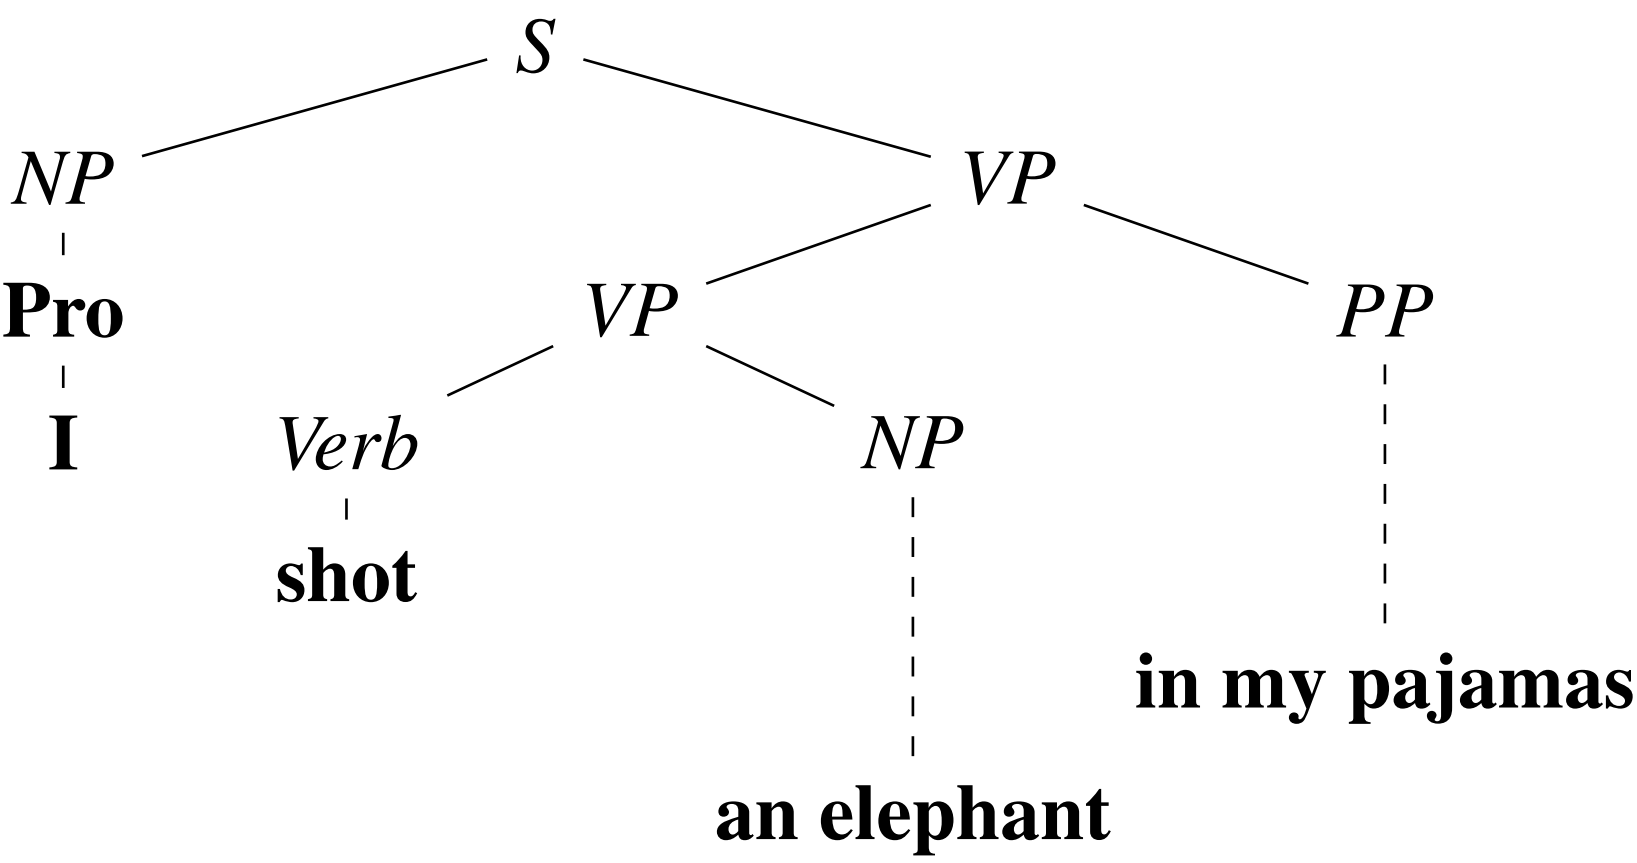
\includegraphics[width=1\textwidth]{imgs/ambiguous-1.png}
\end{subfigure}%
~
\begin{subfigure}{0.5\textwidth}
\centering
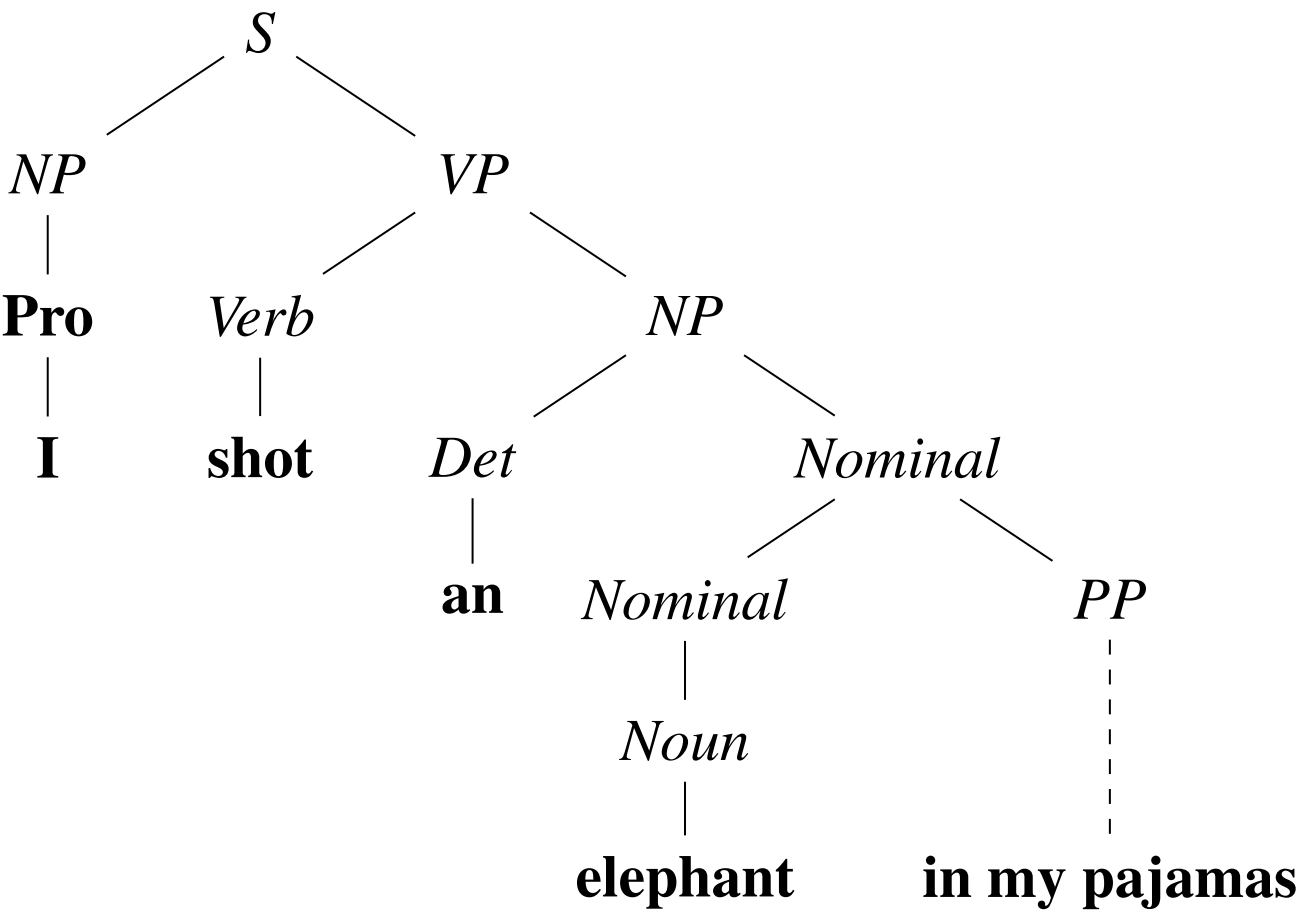
\includegraphics[width=1\textwidth]{imgs/ambiguous-2.png}
\end{subfigure}
\caption{Example of an ambiguous sentence parsing which leads to a different structure where the PP is attached differently.}
\end{figure}

\subsection{Parsing}
\textbf{Recognition}: Given a grammar and input sentence, decide whether the
input is correct \\
\textbf{Parsing}: Given a grammar and input sentence, assign a parse tree
to the sentence

If parsing returns at least one parse tree, then we know the input is also
recognised. Parsing can be seen as a form of search where we are searching
for a tree that is consistent with the grammar and has the input string
as its \textbf{yield}. There are two general approaches to parsing,
\textbf{top-down} and \textbf{bottom-up}.

\subsubsection{Top-down parsing}
In top-down parsing, we start with the start symbol $S$ and work downwards,
expanding the left-most non-terminal first. Problems occur if we start with
the wrong choice where the search will fail.

It is also inefficient for expanding non-terminals without looking at what
is in the given input. For example, given the two rules
\begin{align*}
Nominal &\rightarrow Nominal\ PP \\
Nominal &\rightarrow Noun
\end{align*}
One can keep expanding the $Nominal$, adding a $PP$ each time, without ever
consuming any input and so this will never finish.

\subsubsection{Bottom-up parsing}
In bottom-up parsing, we start from each word and its category, going up and
matching to more categories. This can also make wrong choices, which causes
backtracking and may lead to exponential-time behaviour.

\subsubsection{Cocke-Kasami-Younger (CKY) algorithm}
\begin{itemize}
\item Assumes CFG is in CNF form
\item Works bottom-up
\item Computes subparses for short substrings which are then extended to
larger parses for larger substrings
\end{itemize}

To transform a CFG to CNF, we need to
\begin{itemize}
\item eliminate epsilon rules
\item eliminate unit rules
\item break up long rules
\end{itemize}

For CKY recognition, we assume an input $w$ of length $n$
\begin{enumerate}
\item Let parse table $T = \emptyset$
\item For $i = 1, ..., n$ do:
	\begin{enumerate}
	\item For each rule $A \rightarrow w_i$ add ($i - 1, A, i$) to $T$
	\item For $k = i - 2, ..., 0$ and $j = k+1, ..., i - 1$ do \\
	For each rule $A \rightarrow BC$ and all ($k, B, j$), ($j, C, i$) $\in T$
	add ($k, A, i$) to $T$
	\end{enumerate}
\item Recognise the input if ($0, S, n$) $\in T$
\end{enumerate}

For CKY parsing, we must extend the algorithm and choose between two things:
\begin{itemize}
\item Maintain backpointers to record for each table entry how it arose
\item Read parse trees directly from the existing table
\end{itemize}
\end{document}